This chapter details the comprehensive experimental study conducted to evaluate the performance of the \DPmst\ algorithm. We begin by discussing the test cases, which include experiments on random graphs and how they have been created, real dynamic graphs; and the implementation of a hot start technique to enhance efficiency without compromising results.

Next, we describe the running environment and validate the random graph generator to ensure the reliability of our experiments. The chapter then delves into various aspects of the \DPmst\ design, including input reading, edge ordering, Decoupled Event Handling, filter size, and pre-processing steps.

Following this, we present a comparative analysis of the \DPmst\ algorithm against other algorithms on both static and real dynamic graphs. The section on static graphs examines the performance of parallel algorithms, while the section on real dynamic graphs highlights the effectiveness of the \DPmst\ algorithm in maintaining the \mst\ over time.

Through these experiments, we aim to provide a thorough evaluation of the \DPmst\ algorithm, demonstrating its strengths and identifying areas for further optimization.

\section{Generation of Test Cases}

We have two different suites of test cases. One of synthetic random graphs which are static and the other one of real dynamic graphs.

We generated random graphs where each edge has a probability $p$ of being present of different number of vertices using the Algorithm~\ref{alg:graph}. For each combination of nodes ($10^3, 2\cdot10^3, 10^4, 5\cdot10^4$) and edge probability ($0.10, 0.25, 0.50, 0.75, 0.9$), 20 random graphs were generated. This suite allows to understand different relationships between edges, densities and distribution along the pipeline.

Additionally, we obtained some realistic dynamic graphs (Table~\ref{tab:dyngraphs}) collected by the authors in~\cite{Hanauer2022} and available in \href{https://DynGraphLab.github.io/}{\texttt{https://DynGraphLab.github.io/}}. We had to adapt them to our format and some of them did not have weights or they were artificially generated by the repository, so we added a weight picked uniformly at random in the range 0 to 1.

\begin{table}[H]
\centering
\begin{tabular}{@{}lll@{}}
\toprule
Dataset        & Vertices  & Operations \\ \midrule
amazon-ratings & 495,452   & 476,728     \\
as-caida       & 31,379    & 19,468      \\
frwiki         & 2,212,682 & 31,624,375  \\
movielens10m   & 49,847    & 384,585     \\
simplewiki     & 100,312   & 889,016     \\ \bottomrule
\end{tabular}
\caption{Propoerties of the real dynamic graphs used \label{tab:dyngraphs}}
\end{table}

    \subsection*{Random graphs algorithm \label{sec:exp:rand_graph}}
    A binomial random graph is constructed by connecting labeled nodes randomly with each edge being included in the graph with probability $p$, independently from every other edge. This type of random graphs was presented by Gilbert in~\cite{Gilbert1959}, but the proposed implementation in Algorithm \ref{alg:graph} is based on~\cite{Batagelj2005}. The idea is to generate a random number to determine how many edges to skip based on the probability $p$.
    
    \begin{algorithm}[H]
    \caption{Generating a binomial random graph \label{alg:graph}}
    \begin{algorithmic}
        \Procedure{RandomGraph}{$N, p$}
            \State $G \gets \varnothing$
            \State $v \gets 1$
            \State $u \gets -1$
            \While{$v < N$}
                \State $u \gets u + 1 + \lfloor\frac{\log{(1 - \text{Rand()})}}{\log{(1-p)}}\rfloor$
                \While{$u \geq v \land v < N$}
                    \State $u \gets u - v$
                    \State $v \gets v + 1$
                \EndWhile
                \If{$v < N$}
                    \State $G \gets G \cup \{(u,v)\}$
                \EndIf
            \EndWhile
            \State \Return $G$
        \EndProcedure
    \end{algorithmic}
    \end{algorithm}

    \subsection*{Random generator validation}
    Our graphs and operations generator utilizes the \Go\ programming language's \verb|math/rand| package. This package employs the ChaCha8 algorithm, a well-regarded stream cipher designed by Daniel Bernstein~\cite{bernstein2008chacha}. The generator produces 63-bit numbers which are then scaled by dividing by $2^{63}$, resulting in uniformly distributed random numbers between 0 and 1. Further details on the internal workings of the generator can be found on the \Go\ Blog\footnote{\href{https://go.dev/blog/randv2}{https://go.dev/blog/randv2}}.
    
    To ensure the quality and reliability of this pseudo-random number generator, we conducted several validation tests. We generated over a million random numbers using the seed `1707242827149724922' and performed two statistical tests: the Chi-square test and the Kolmogorov-Smirnov test.
    
    The Chi-square test~\cite{MacLaren1965,Knuth_1997} is a statistical method used to compare the distribution of a sample of random numbers to an expected uniform distribution. This test involves dividing the range of possible values into several bins, counting the number of random numbers that fall into each bin, and then computing the Chi-square statistic to assess how well the observed distribution matches the expected distribution. A p-value is then calculated; in our case, we used a significance level of 0.05. If the p-value is below this threshold, we reject the null hypothesis that the numbers are uniformly distributed. Our test results indicated no rejection with a p-value of 0.001, confirming that the distribution of our generated numbers was consistent with uniformity at the 0.05 significance level.
    
    The Kolmogorov-Smirnov (K-S) test is another statistical test used to compare a sample distribution to a reference probability distribution (in our case, the uniform distribution)~\cite{Massey1951,Knuth_1997}. This test calculates the maximum distance between the empirical distribution function of the sample and the cumulative distribution function of the reference distribution. A p-value is then derived from this maximum distance. For our generated numbers, we performed the K-S test and obtained a p-value of 0.02. Since this p-value is above the common significance threshold of 0.05, we do not reject the null hypothesis, indicating that our random number generator produces numbers that follow the expected uniform distribution.
    
    Both the Chi-square test and the Kolmogorov-Smirnov test results validate the high quality and reliability of the \verb|math/rand| pseudo-random number generator in Go for our application needs.

    \subsection*{Hot start}
    In our experimental study, we implemented two additional operations in the \DPmst\ algorithm specifically for static graph testing: {\tt savestate} saving the current state of the filters and {\t loadstate} loading this saved state. These operations enable what we term a "Hot Start", allowing the algorithm to resume from a pre-saved state rather than initializing from scratch for each test run. This method significantly enhances efficiency during experimentation without compromising the validity of the results. By using Hot Starts, we can isolate the performance of the algorithm itself from the overhead of repeated initializations, providing a clearer assessment of the algorithm's behavior under various conditions.

    These test cases were designed to evaluate the performance improvements achieved by the optimizations in \DPmst\ and to ensure that the results are both accurate and reproducible.


\section{Analysis of \DPmst\ Architecture and Optimizations}
    In this section, we delve into the experimentation and optimization of the \DPmst\ algorithm. Through a series of tests, we examine various design elements including input handling, edge ordering, event decoupling, filter sizing, and pre-processing. Our goal is to refine the pipeline architecture and enhance its performance for computing and maintaining the \mst.

    \subsection*{Read Input \label{sec:exp:input}}
    As discussed in Section~\ref{sec:dp:input}, \Go\ provides two standard library packages for handling program input and output. The \verb|fmt| package implements formatted I/O with functions similar to C's printf and scanf, while the \verb|bufio| package implements buffered I/O. \verb|bufio| wraps an io.Reader or io.Writer object, creating another object (Reader or Writer) that also implements the interface but adds buffering and assists with textual I/O.

    Since \verb|bufio| uses buffers to read from a file and includes specific readers for various data types without needing a parser to infer the format as scanf does, it intuitively offers better performance than \verb|fmt|. To verify this, we generated a file with the same format as our input graphs and measured the time taken to read it. This experiment was repeated 100 times to obtain stable time measurements.

    Figure~\ref{fig:input-test} shows that, as expected, \verb|bufio| outperformed \verb|fmt|. On average, \verb|bufio| required around 1.04 microseconds per line, whereas \verb|fmt| needed 18.69 microseconds per line. This indicates that using \verb|bufio| instead of \verb|fmt| resulted in a speed-up of approximately 18 times. Consequently, due to these results, \verb|bufio| was chosen for our implementation.

    \begin{figure}[H]
        \centering
        \includegraphics[width=0.8\textwidth]{figures/input_test.eps}
        \cprotect\caption{Running time comparison between \verb|bufio| and \verb|fmt|}
        \label{fig:input-test}
    \end{figure}

    
    \subsection*{Edge order \label{sec:edge_order}}
    We observed that the ordering of the vertices in an edge has a significant impact on the overall performance of the system. Several possible orderings can be proposed, such as a random order of the vertices, a lexicographical increasing order, or an order based on the vertex that has appeared the least number of times, and many more. Each of these strategies or heuristics has its own advantages and complexities.
    
    For our analysis, we focused on two ordering methods: random order and lexicographical order. These methods were chosen because they are relatively simple to implement and do not require prior knowledge of the graph's history. Instead of performing the analysis on the complete \DPmst, we created a simplified model to simulate the behavior of the pipeline. This model allowed us to count where each filter ended up and provided insights into the performance impact of each ordering strategy. The code used for simulate can be found in Appendix~\ref{appendix:dp_sim:rand} and Appendix~\ref{appendix:dp_sim:real}.

    Figure~\ref{fig:density:random} illustrates the simulation results for a random graph with 100,000 vertices and a density of 0.9. Figure~\ref{fig:density:real} shows the simulation results for a real dynamic graph with 2,212,682 vertices and 31,624,375 operations. In both cases, we observed that the lexicographical order resulted in fewer filters, which helps to reduce the overhead associated with managing multiple goroutines. However, this reduction in filters comes at a cost: the remaining filters tend to accumulate more edges, leading to more costly operations.
    
    The results indicate that while the lexicographical order can help streamline the pipeline by reducing the number of filters, it can also increase the workload on each filter. This trade-off highlights the importance of carefully choosing the vertex ordering strategy based on the specific characteristics and requirements of the application. Further research and experimentation may reveal additional strategies that balance these trade-offs more effectively. But at this point of time, we chose the lexicographical order for the rest of the experiments.
    
    At this point in time, we chose the lexicographical order for the rest of the experiments. This decision was based on its demonstrated ability to minimize the number of filters, thereby reducing the goroutine overhead despite the increased workload on each filter.
    
    \begin{figure}
        \centering
        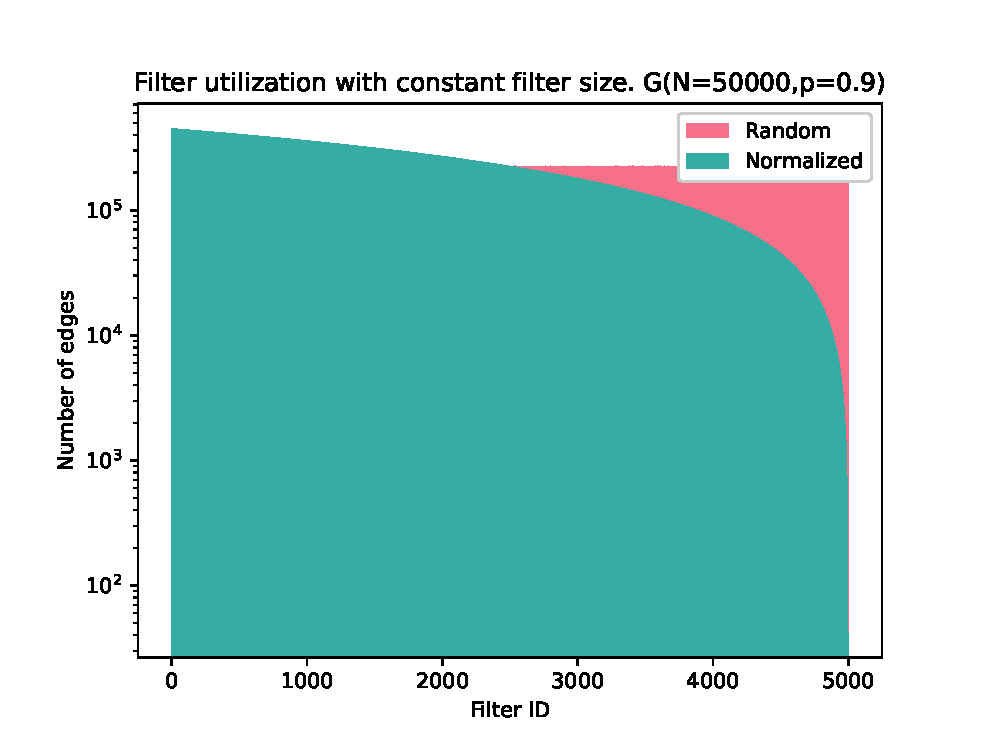
\includegraphics[width=0.9\linewidth]{figures/DP_Densities_random}
        \caption{Simulation of the \DPmst\ with 10 roots per filter using a random graph.}
        \label{fig:density:random}
    \end{figure}
    
    \begin{figure}
        \centering
        \includegraphics[width=0.9\linewidth]{figures/DP_Densities.pdf}
        \caption{Simulation of the \DPmst\ with 10 roots per filter using a real dynamic graph.}
        \label{fig:density:real}
    \end{figure}

    
    \subsection*{Decoupled Event Handling}
    As detailed in Section~\ref{sec:dp:decouple}, the MailBox/Worker optimization, termed ``Decoupled Event Handling", was introduced to address inefficiencies in the original filter stage implementation. By separating the event handling and processing responsibilities into distinct stages —the MailBox and the Worker- we aimed to enhance the overall performance and responsiveness of the system.

    To evaluate the impact of this optimization, we conducted an experiment that involved generating files of different sizes and measuring the execution time with and without the optimization. The results are shown in Table~\ref{tab:messenger}. For a file with 7,500 random requests, we observed a speed-up of 20\% with the optimization. When the file size increased to 10,000 random requests, the speed-up increased to 38\%. These results clearly indicate that the optimization significantly reduces the locking of the pipeline, allowing for more efficient processing as the number of operations increases. The more operations there are, the more pronounced the performance improvement becomes, demonstrating the effectiveness of the MailBox/Worker optimization in handling larger workloads and enhancing system throughput.

    \begin{table}[H]
    \centering
    \begin{tabular}{@{}lrr@{}}
    \toprule
    Operations & No optimization & With optimization \\ \midrule
    7500       & 1h 9m 31.48s    & 57m 28.23s        \\
    10000      & 3h 46m 46.73s   & 2h 44m 14.19s     \\ \bottomrule
    \end{tabular}
    \caption{Execution time of \DPmst\ of different file sizes with and without the MailBox/Worker optimization.\label{tab:messenger}}
    \end{table}
            
    \subsection*{Filter size \label{sec:filter_size}}
    As mentioned in Section~\ref{sec:dp:fsize}, having multiple roots per filter can lead to a more efficient utilization of computational resources, but it also brings an additional parameter that can affect the performance of the \DPmst.

    To study the effect of the number of roots in each filter, we consider three options: a constant number of roots \DPmstv{const},  $\log(n)$ roots \DPmstv{log}, and $\sqrt{n}$ roots \DPmstv{sqrt} (where $n$ is the number of vertices of the input graph). We will initialize the \DPmst\ and then measure the performance in a single core machine in order to compare their behaviour.

    Figure~\ref{fig:Fsize_comparison} shows the corresponding experimental results. We can observe that, as expected, this value influences the performance of the algorithm. For small graphs it seems that the version that works with filters with a $\sqrt{n}$ number of roots is better and faster than the others, but as the graph becomes larger and denser the versions with a logarithmic or even constant number of roots per filter become more efficient.
        
    \begin{figure}[H]
    \begin{center}
        \includegraphics[width=\textwidth]{figures/SomeDensities_mixed.pdf}
    \end{center}
    \caption{A comparison of three versions of the \DPmst\ algorithm varying the number of roots at each filter: \DPmstv{const}, \DPmstv{log} and \DPmstv{sqrt}\ with a single core\label{fig:Fsize_comparison}}
    \end{figure}

    This trend is more evident when we group the results by different densities and the expected number of edges, computed as $n \cdot (n-1) \cdot p$. Figure~\ref{fig:Fsize_comparison_edges} illustrates that there is a clear point at which the efficiency of the $\log(n)$ and constant root versions surpasses that of the $\sqrt{n}$ version. This transition point depends on the graph size and density, highlighting the importance of choosing an appropriate number of roots based on the specific characteristics of the input graph.

    \begin{figure}
        \centering
        \includegraphics[width=0.7\linewidth]{figures/FilterSizeExpectedEdges.pdf}
        \caption{A comparison of three versions of the \DPmst\ algorithm varying the number of roots at each filter and focusing on the number of edges: \DPmstv{const}, \DPmstv{log} and \DPmstv{sqrt}\ with a single core\label{fig:Fsize_comparison_edges}}
    \end{figure}

    
    \subsection*{Pre-processing}
    Some experimental work \cite{Amato1997,cattaneo2010,Iyer2001,Frederickson1985} comparing different algorithms to maintain a dynamic \mst\ involves a pre-processing step, which is typically considered insignificant. These studies often compare data structures based on Euler Trees~\cite{Sleator1983}, which require vertices to have a maximum degree of 3. To meet this requirement, vertices with a degree greater than 3 are ``exploded" into multiple vertices, equal to the initial vertex's degree, and connected in a loop with edges of weight 0. This ensures that all but one edge will be added during processing. An example of this process is shown in Figure~\ref{fig:preprocess:example}.

    \begin{figure}
        \centering
        \resizebox{0.8\textwidth}{!}{
        \begin{tikzpicture}
    \node[shape=circle,draw=black, fill = blue!30] (center) at (0,0) {$v$};
    
    % Define the radius of the pentagon
    \def\radius{3}
    \def\N{5}

    % Utils:
    \pgfmathtruncatemacro{\polystep}{360 / \N}
    \pgfmathtruncatemacro{\range}{\N - 1}
    
    % Define the coordinates for the pentagon vertices
    \foreach \i in {0,...,\range}
    {
        \node (v\i) at ({\radius*cos(90+\i*\polystep)},{\radius*sin(90+\i*\polystep)}) {};
    }

    % Connect with the center
    \foreach \i in {0,...,\range}
    {
        \pgfmathtruncatemacro{\weight}{\i + 1}
          \draw[-, draw=black] (center) to["\weight"] (v\i);
    }
\end{tikzpicture}
\begin{tikzpicture}
    
    % Define the radius of the pentagon
    \def\radius{1.5}
    \def\N{5}

    % Utils:
    \pgfmathtruncatemacro{\polystep}{360 / \N}
    \pgfmathtruncatemacro{\range}{\N - 1}
    
    % Define the coordinates for the pentagon vertices
    \foreach \i in {0,...,\range}
    {
        \node[shape=circle,draw=black, fill = blue!30] (v\i) at ({\radius*cos(90+\i*\polystep)},{\radius*sin(90+\i*\polystep)}) {$v_\i$};
    }
    
    % Define the coordinates for the external vertices
    \foreach \i in {0,...,\range}
    {
        \node (w\i) at ({2*\radius*cos(90+\i*\polystep)},{2*\radius*sin(90+\i*\polystep)}) {};
    }

    % Connect to external
    \foreach \i in {0,...,\range}
    {
        \pgfmathtruncatemacro{\weight}{\i + 1}
          \draw[-, draw=black] (v\i) to["\weight"] (w\i);
    }

    % Connect in ring
    \foreach \i in {0,...,\range}
    {
        \pgfmathtruncatemacro{\iplusone}{mod(\i + 1, \N) }
          \draw[-, draw=black] (v\i) to["0"] (v\iplusone);
    }

\end{tikzpicture}}
        \caption{Example of the pre-processing step on a vertex with degree 5.\label{fig:preprocess:example}}
    \end{figure}

    To verify the insignificance of this pre-processing step and to determine whether the \DPmst\ could benefit from it, we conducted our own experiments. Figure~\ref{fig:preprocess} demonstrates that this pre-processing step actually results in a higher initialization time compared to processing without it. For instance, in a binomial graph originally consisting of 1000 vertices with a density of 0.75, transforming the graph so that no vertex has a degree greater than 3 resulted in a 100\% slow-down (The average time with preprocess divided by the time without it). Similarly, for a graph with 7500 vertices and the same density, this transformation led to a 75\% slow-down.

    These results indicate that the pre-processing time is not negligible and that this approach is not advantageous for the \DPmst.

    \begin{figure}[H]
    \begin{center}
        \includegraphics[width=0.77\textwidth]{figures/preprocess.eps}
    \end{center}
    \caption{Comparison of \DPmst\ initialization with and without preprocessing. \label{fig:preprocess}}
    \end{figure}
    
\section{Comparison with other algorithms}
    In this section, as usual in parallel applications~\cite{bader2002algorithm} we have captured  the elapsed wall-clock time $T(k,n,p)$, which is the time elapsed from the moment in which the first processor started working to the moment in which the last processor completed the computation for a graph of  $n$ vertices and expected density of $p$ using $k$ processors. We will refer to absolute speed up and efficiency as: 
    \begin{itemize}
        \setlength\itemsep{-0.5em}
        \item \textit{Absolute speedup}: $speedup_a(k) = T(1, n, p)/T(k, n, p)$.
        \item \textit{Efficiency}: $speedup_a(k)/k$.
    \end{itemize} 
    where $T(1, n, p)$ is the execution time of the \mst\ sequential implementation.
    
    \subsection*{Static graphs}
        In Figure \ref{fig:others_algorithms}, we compare the performance of the Dynamic Pipeline (\DPmst) against the standard Kruskal algorithm and the Filter-Kruskal (\FKruskal) algorithm, as explained in Section \ref{sec:filter_kruskal}. The results clearly demonstrate that \DPmst\ offers a significant reduction in execution time across all graph densities. This indicates that the partitioning strategy utilized by \DPmst\ is highly effective, providing superior performance regardless of the density of the graph. This efficiency is evident from the consistently lower execution times of \DPmst\ compared to {\tt Kruskal}.
    
        \begin{figure}
        \begin{center}
            \includegraphics[width=\textwidth]{figures/Others.pdf}
        \end{center}
        \caption{A comparison of DP-MST with different algorithms with a single core.}
        \label{fig:others_algorithms}
        \end{figure}

    
        \subsubsection*{Parallel algorithms:}
        
        If we focus on the algorithms that can be easily parallelized, we compare \DPmst\ with our implementation of \FKruskal\ and the results presented in~\cite{Lonar2014} of an implementation of {\tt Prim} using message-passing parallelism. In Figure~\ref{fig:static:multiples}, we can observe that {\tt Prim} is far from optimal. Although \FKruskal\ is faster at the beginning, for larger graphs it is easily outperformed by \DPmst. This comparison highlights the superior scalability and efficiency of \DPmst\ in handling large, dynamic graphs. Our experiments demonstrate that while \FKruskal\ can provide competitive performance on smaller datasets, its efficiency diminishes as the graph size increases. 

        \begin{figure}
            \centering
            \includegraphics[width=1\linewidth]{figures/SomeDensities_mixed.pdf}
            \caption{\label{fig:dpmst-versions}Comparison of \DPmst\ with \DPmstv{const(10)}, \DPmstv{log}, \DPmstv{sqrt}, {\tt Prim} and \FKruskal\ on a single core.}
            \label{fig:static:multiples}
        \end{figure}
        
        In evaluating the performance of \DPmst\ and \FKruskal\ on random graphs, the experimental results reveal significant insights into the scalability and efficiency of these algorithms. By examining the speed-up achieved with an increasing number of cores, as illustrated in Figure~\ref{fig:static:speedup}, we observe that \DPmst\ consistently demonstrates superior parallel performance compared to \FKruskal. For instance, in graphs with varying sizes and densities —such as $G(n=1000,p=0.25)$,  $G(n=5000,p=0.75)$, and $G(n=10000,p=0.90)$— \DPmst\ exhibits substantial speed-ups across all configurations. Notably, \DPmst\ with a logarithmic number of roots per filter (\DPmstv{log}) achieves near-linear speed-up and almost a perfect efficiency (Figure~\ref{fig:static:efficiency}) as the number of cores increases, highlighting its effectiveness in leveraging parallelism. In contrast, while \FKruskal\ also benefits from parallel execution, its performance gains are comparatively modest, particularly for larger and denser graphs. This underscores the efficiency of the \DPmst\ architecture in distributing computational workload and minimizing synchronization overhead, thereby making it a highly scalable solution for computing \mst\ in parallel environments.
        
        \begin{figure}
            \centering
            \includegraphics[width=1\linewidth]{figures/SpeedUpDPandFK_sample.pdf}
            \caption{Speed-up comparison of \DPmst\ and \FKruskal}
            \label{fig:static:speedup}
        \end{figure}
        
        \begin{figure}
            \centering
            \includegraphics[width=1\linewidth]{figures/EfficiencyDPandFK.pdf}
            \caption{Efficiency comparison of \DPmst\ and \FKruskal}
            \label{fig:static:efficiency}
        \end{figure}
    \subsection*{Real dynamic graphs}
    We compare \DPmst\ and \FKruskal\ on realistic dynamic graphs to evaluate their performance in maintaining the minimum spanning tree (\mst) after each edge insertion or deletion. For each operation, we request an update of the \mst\ to assess how efficiently the algorithms handle dynamic changes.
    
    In Table \ref{tab:real_graphs_time}, we observe that \DPmst\ effectively maintains the \mst\ across various datasets. This table highlights the execution times for different graph sizes and densities, illustrating how \DPmst\ consistently outperforms \FKruskal\ in maintaining the \mst.

    Figure \ref{fig:real_graphs_speed} further demonstrates the scalability and efficiency of \DPmst\ in a parallel processing environment. By leveraging the parallelism capabilities inherent in its design, \DPmst\ achieves significant speed-ups, especially as the number of processing cores increases. This figure clearly shows that \DPmst\ scales well with the addition of more cores, maintaining its performance advantage over \FKruskal\ even as the computational load grows.

    These results underscore the robustness and efficiency of \DPmst\ in real-world scenarios, where dynamic updates to the \mst\ are frequent and computational resources need to be optimally utilized. The combination of effective maintenance of the \mst\ and superior scalability in parallel environments makes \DPmst\ a compelling choice for handling dynamic graph problems in various applications.
    
    \begin{figure}
        \centering
        \begin{subfigure}{\textwidth}
         \centering
            \begin{tabular}{lrr}
                \toprule
                Dataset            & \FKruskal & \DPmst\   \\ \midrule
                {\tt as-caida}     &  1h 30min &  1h 19min \\
                {\tt movielens10m} &  1h 39min &  1h 20min \\
                {\tt simplewiki}   & 17h  8min & 11h 29min \\
                \bottomrule
            \end{tabular}
            \caption{\label{tab:real_graphs_time}Execution time comparison with 1 core and 10 roots per filter}
        \end{subfigure}
        \centering
        \begin{subfigure}{\textwidth}
        \centering
            \includegraphics[width=\textwidth]{figures/RealGraphs.pdf}
            \caption{\label{fig:real_graphs_speed}Comparison of speed-ups in a multicore set-up}        
       \end{subfigure}
        \caption{\label{fig:real-graphs}Experimental results on real dynamic graphs.}
    \end{figure}


\section{Running environment}

Experiments  were run at the cluster of the 
RDLab-UPC (\href{https://rdlab.cs.upc.edu/}{\texttt{https://rdlab.cs.upc.edu/}})
on different nodes with the processors Intel(R) Xeon(R) CPU X5675 @ 3.07GHz and 12 cores, Intel(R) Xeon(R) CPU X5670 @ 2.93GHz and 12 cores, Intel(R) Xeon(R) CPU X5660 @ 2.80GHz and 12 cores, Intel(R) Xeon(R) CPU X5550 @ 2.67GHz and 8 cores, and Intel(R) Xeon(R) CPU E5-2450 @ 2.50GHz and 16 cores. The configuration used for submitting jobs was up to 16GB of RAM and a maximum number of cores depending on the experiment. The same job was executed 10 times and the average was reported. The timeout was 24 hours.